%
% Author: Riccardo Orizio
% Date: Wed 17 May 2017
% Description: Presentation for United Technologies Research Center
%

\documentclass{beamer}

\usepackage[utf8]{inputenc}
\usepackage{graphicx}
\usepackage{amsmath}

\graphicspath{ {./Images/} }

% Style properties
\usetheme{Warsaw}
\usefonttheme{structuresmallcapsserif}
\usefonttheme{professionalfonts}
\usecolortheme{seahorse}

% Defining a unique space modifier, mostly used in the itemize environment
\def\itemizespace{\vspace{7mm}}

% Title page information
\title[UTRC]{Diagnosis on embedded systems}
\author[Orizio]{Riccardo Orizio}
\institute[UCC]
{
	Prof. Gregory Provan\\
	\vspace{2mm}
	Department of Computer Science\\
	\vspace{1mm}
	University College Cork\\
}
\date[2017]{16 May 2017}
\titlegraphic{
\includegraphics[width=0.15\textwidth]{logo_ucc.png}}


\begin{document}

\begin{frame}
	\titlepage
\end{frame}

% Table of contents?

\section{Problem}
\subsection{Problem definition}
\begin{frame}{Three tanks}
	Diagnosis of errors in high-fidelity models using a data-driven approach
	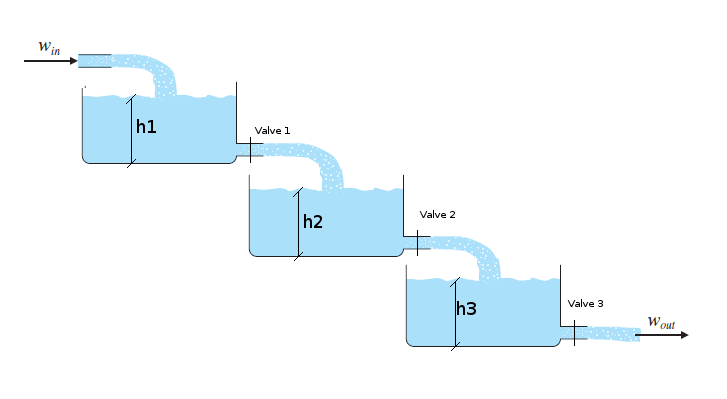
\includegraphics[width=0.9\textwidth]{3tanks.png}
\end{frame}

\begin{frame}{Three tanks}
	\begin{description}
		\item[Differential equation:]
			$
			\begin{aligned}
				\delta(h_i) = \frac{ in_i - out_i }{ h_{max} }
			\end{aligned}
			$
			\itemizespace%

		\item[Non Linear model:] \hfill \vspace{3mm}
			$
			\begin{aligned}
				out_i = \text{Valve}_i \cdot \sqrt{ \max{( 0, 2 \cdot g \cdot h_{max} \cdot (h_i - h_{i+1} ) ) } }
			\end{aligned}
			$
			\itemizespace%

		\item[Linear model:] \hfill \vspace{3mm}
			$
			\begin{aligned}
				out_i = \text{Valve}_i \cdot \max{( 0, 2 \cdot g \cdot h_{max} \cdot (h_i - h_{i+1}) ) }
			\end{aligned}
			$
	\end{description}
\end{frame}

\begin{frame}{Three tanks simulation}
	\begin{figure}
		\centering
		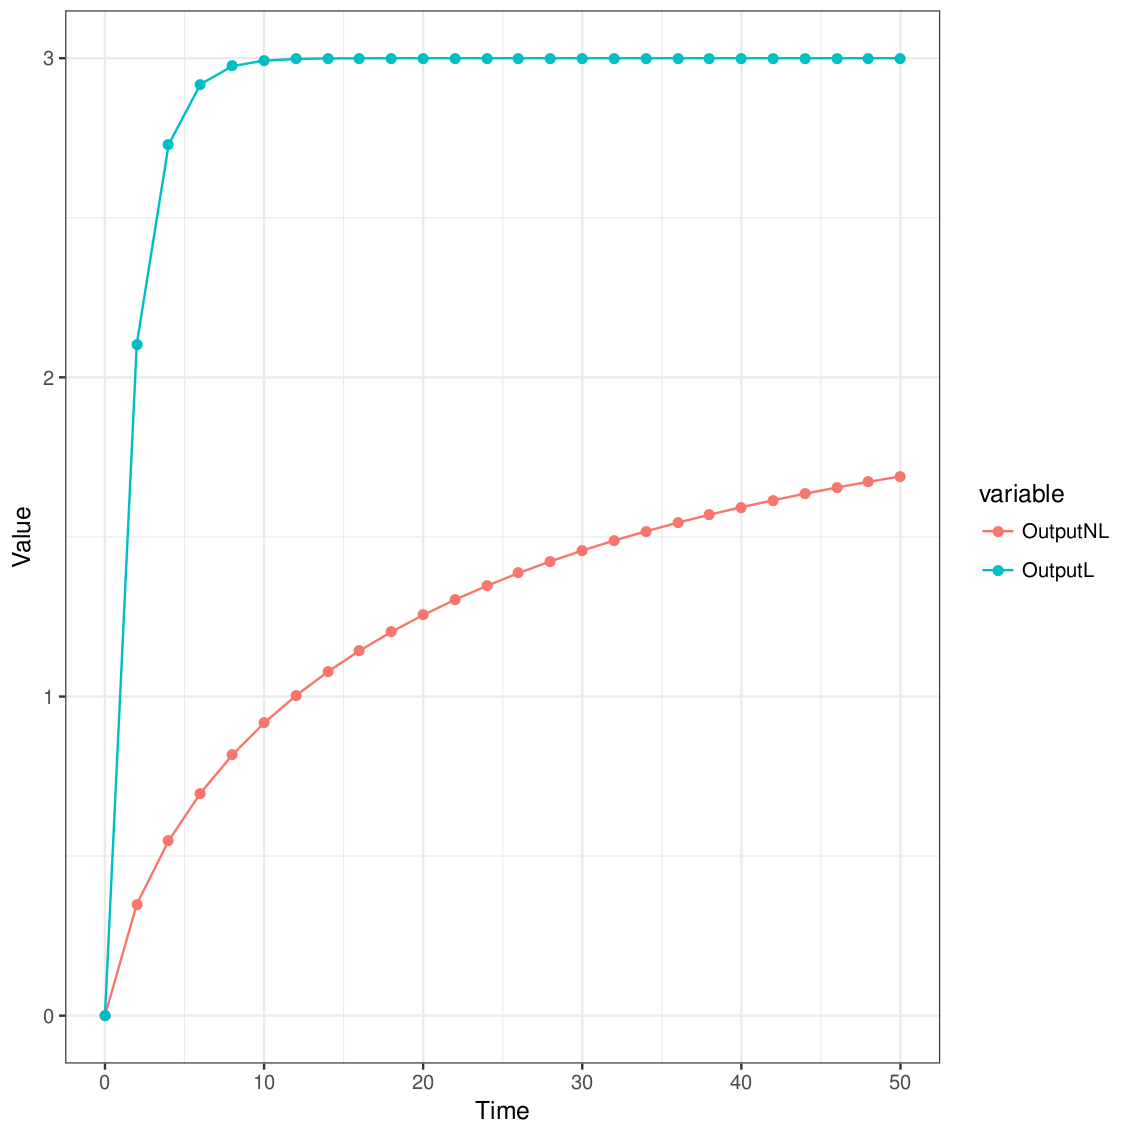
\includegraphics[height=0.8\textheight]{3tanks_simulation.png}
	\end{figure}
\end{frame}

\subsection{Solution}
\begin{frame}{Correction function}
	\begin{figure}
		\centering
		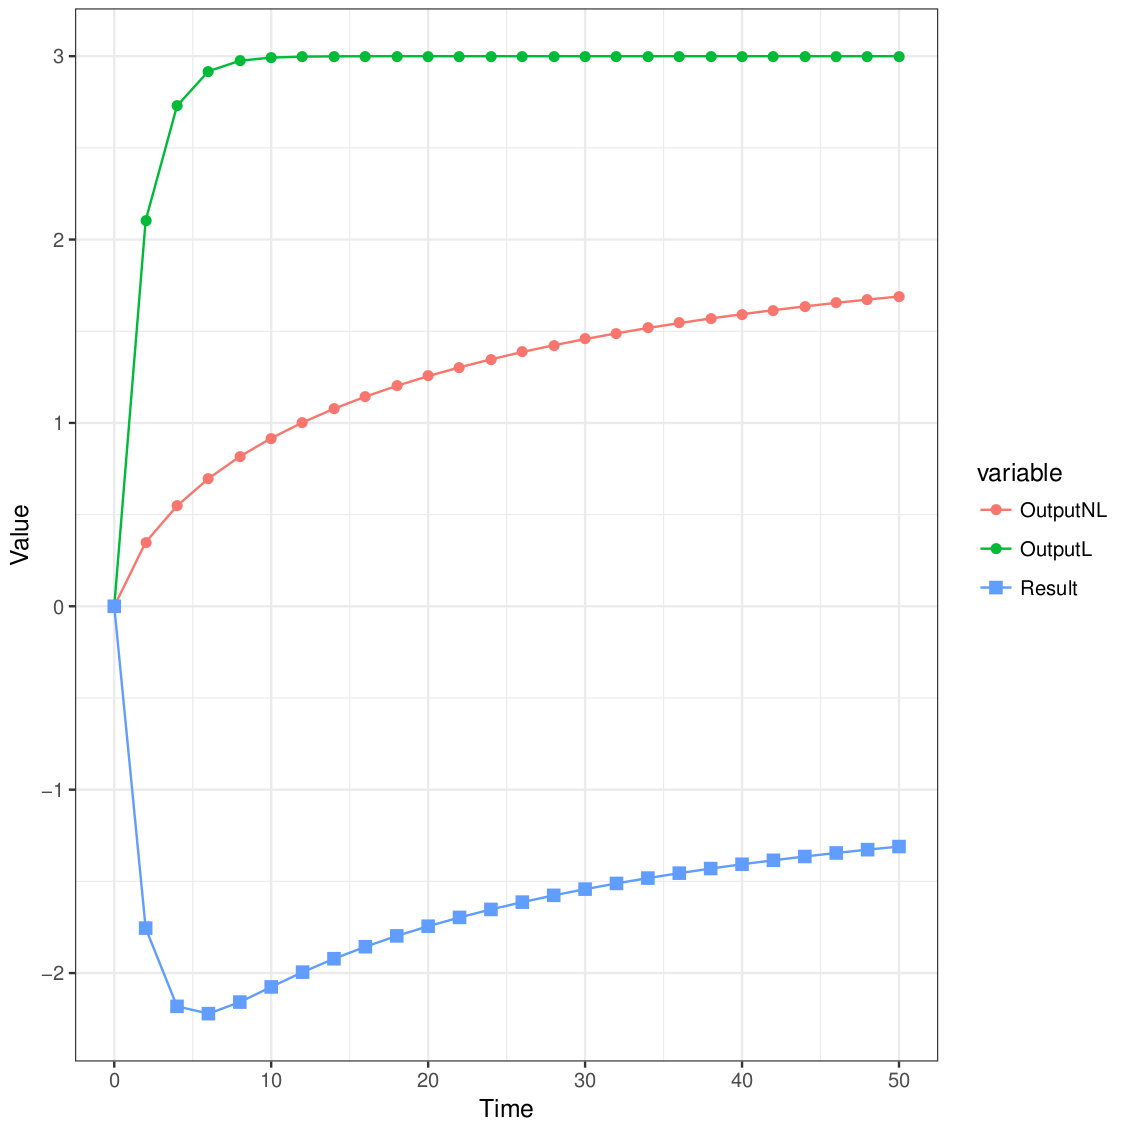
\includegraphics[height=0.8\textheight]{3tanks_correction.png}
	\end{figure}
\end{frame}

\section{Issues}
\subsection{Types of problems}
\begin{frame}{Types of problems}
	\begin{itemize}[<+->]
		\item[-] Valve problems
		\itemizespace%

		\item[-] Different type of inputs
		\itemizespace%

		\item[-] Combinations of the above
	\end{itemize}
\end{frame}

\begin{frame}{Valve problems}
	\begin{table}
		\begin{tabular}{ cc }
			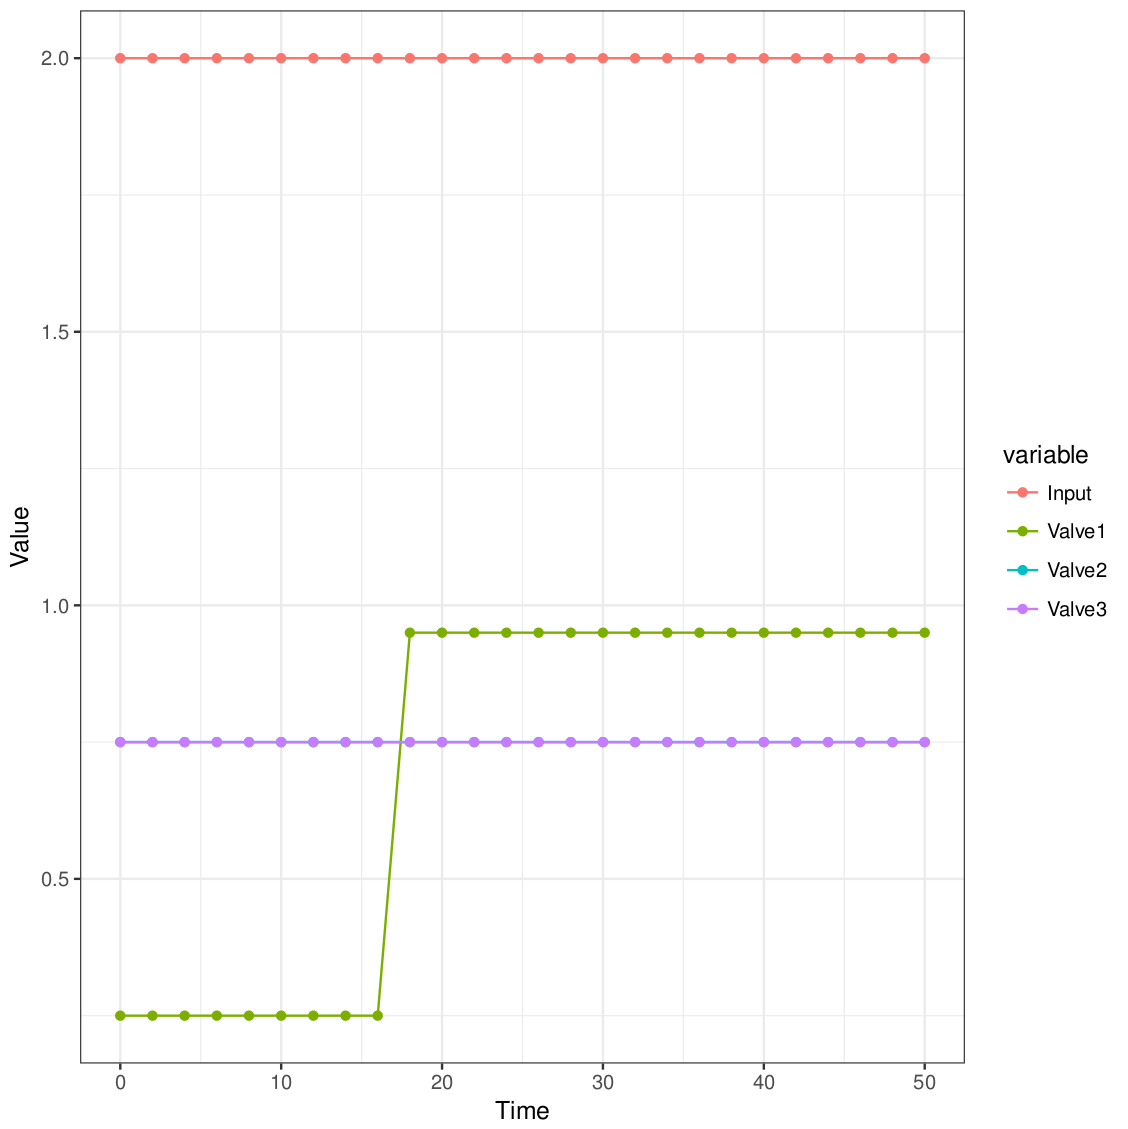
\includegraphics[width=0.5\textwidth]{issues_v1_input.png} &
			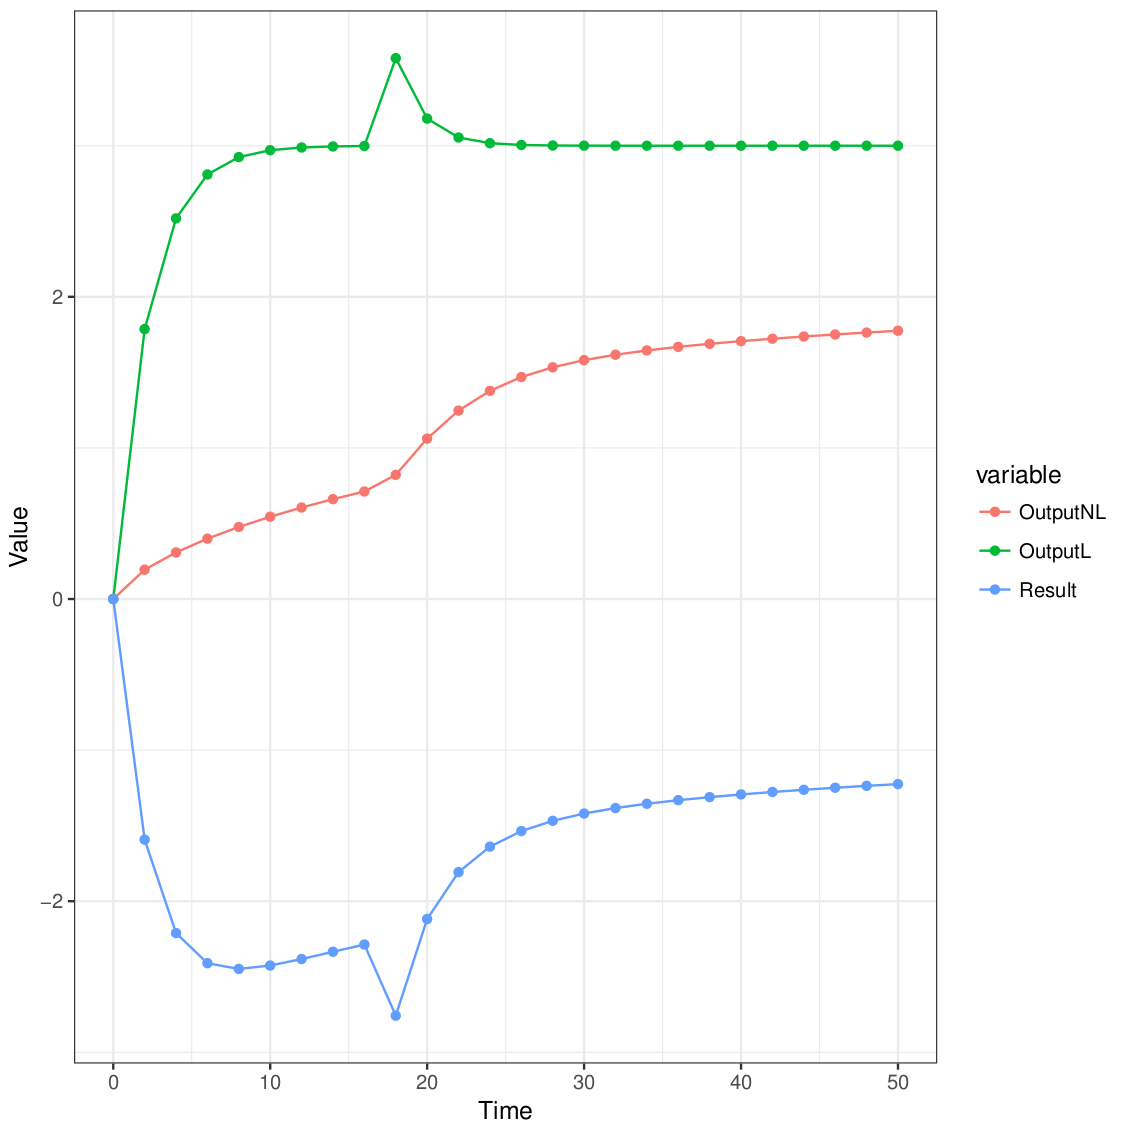
\includegraphics[width=0.5\textwidth]{issues_v1_output.png} \\
		\end{tabular}
	\end{table}
\end{frame}

\begin{frame}{Different inputs}
	\begin{table}
		\begin{tabular}{ cc }
			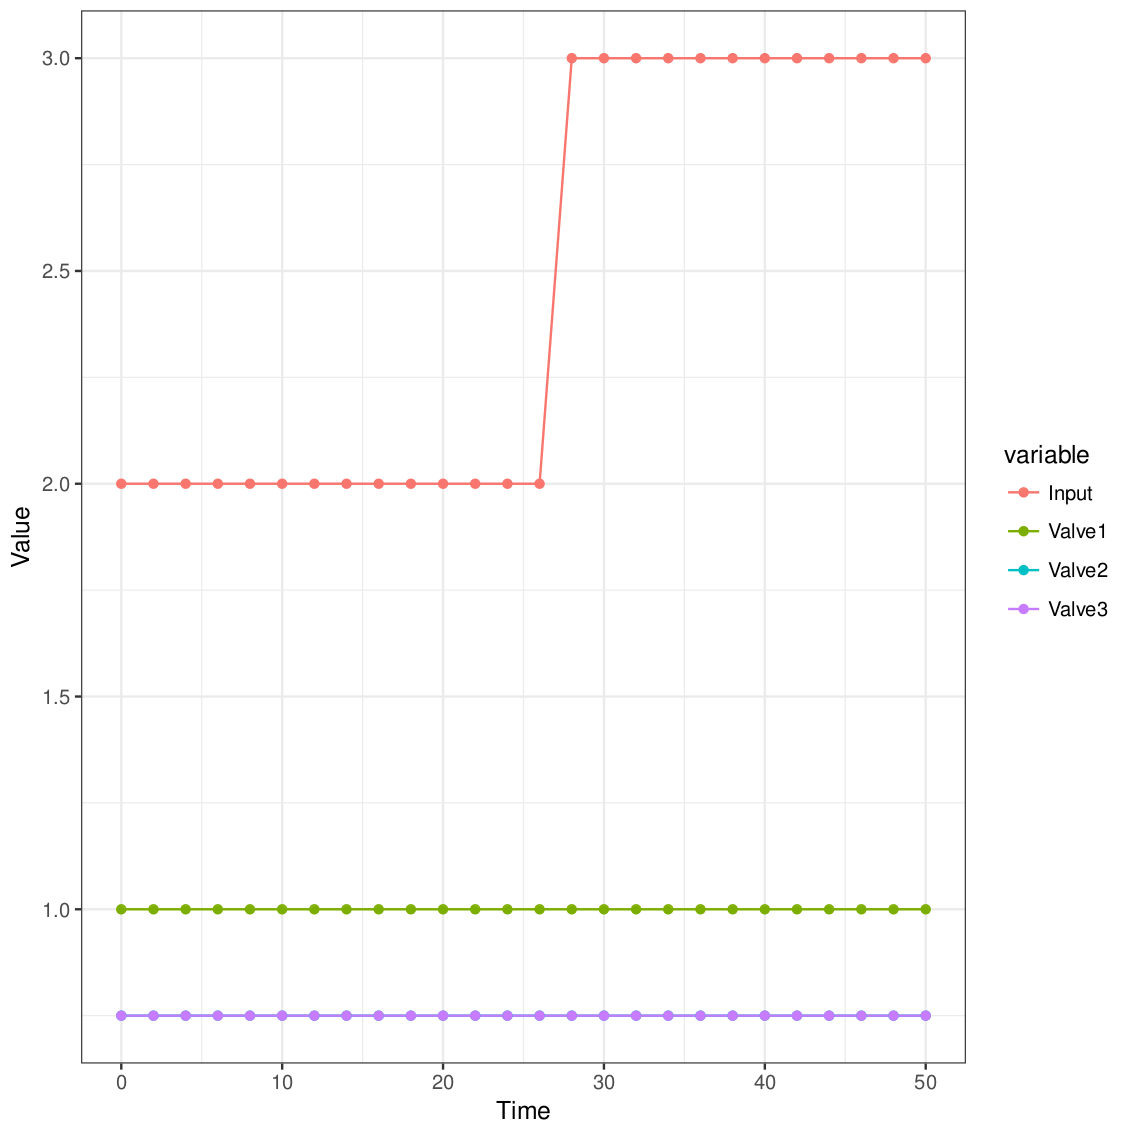
\includegraphics[width=0.5\textwidth]{issues_step_input.png} &
			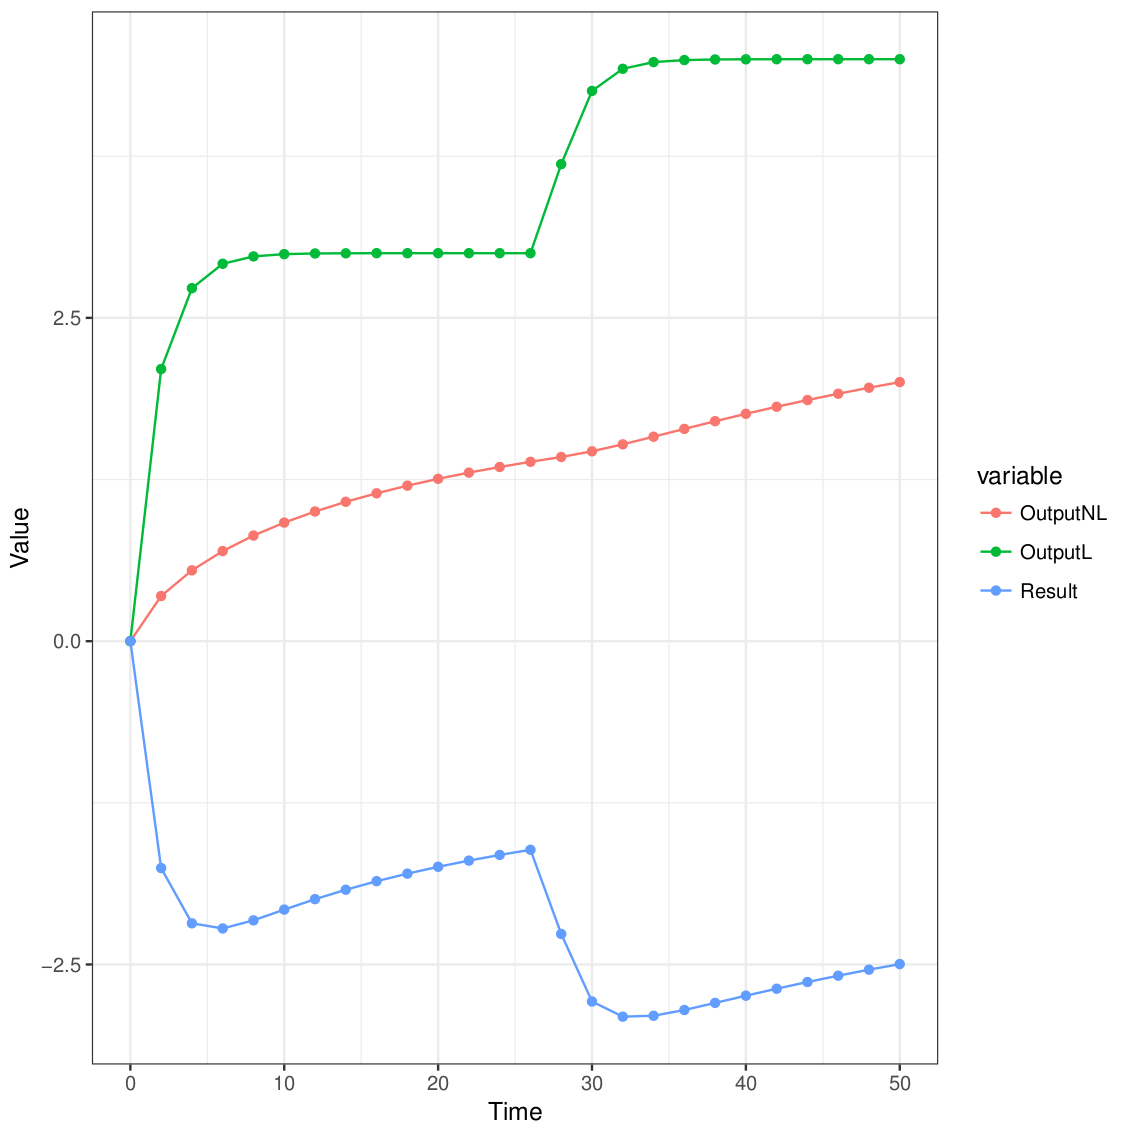
\includegraphics[width=0.5\textwidth]{issues_step_output.png} \\
		\end{tabular}
	\end{table}
\end{frame}

\begin{frame}{Combinations of issues}
	\begin{table}
		\begin{tabular}{ cc }
			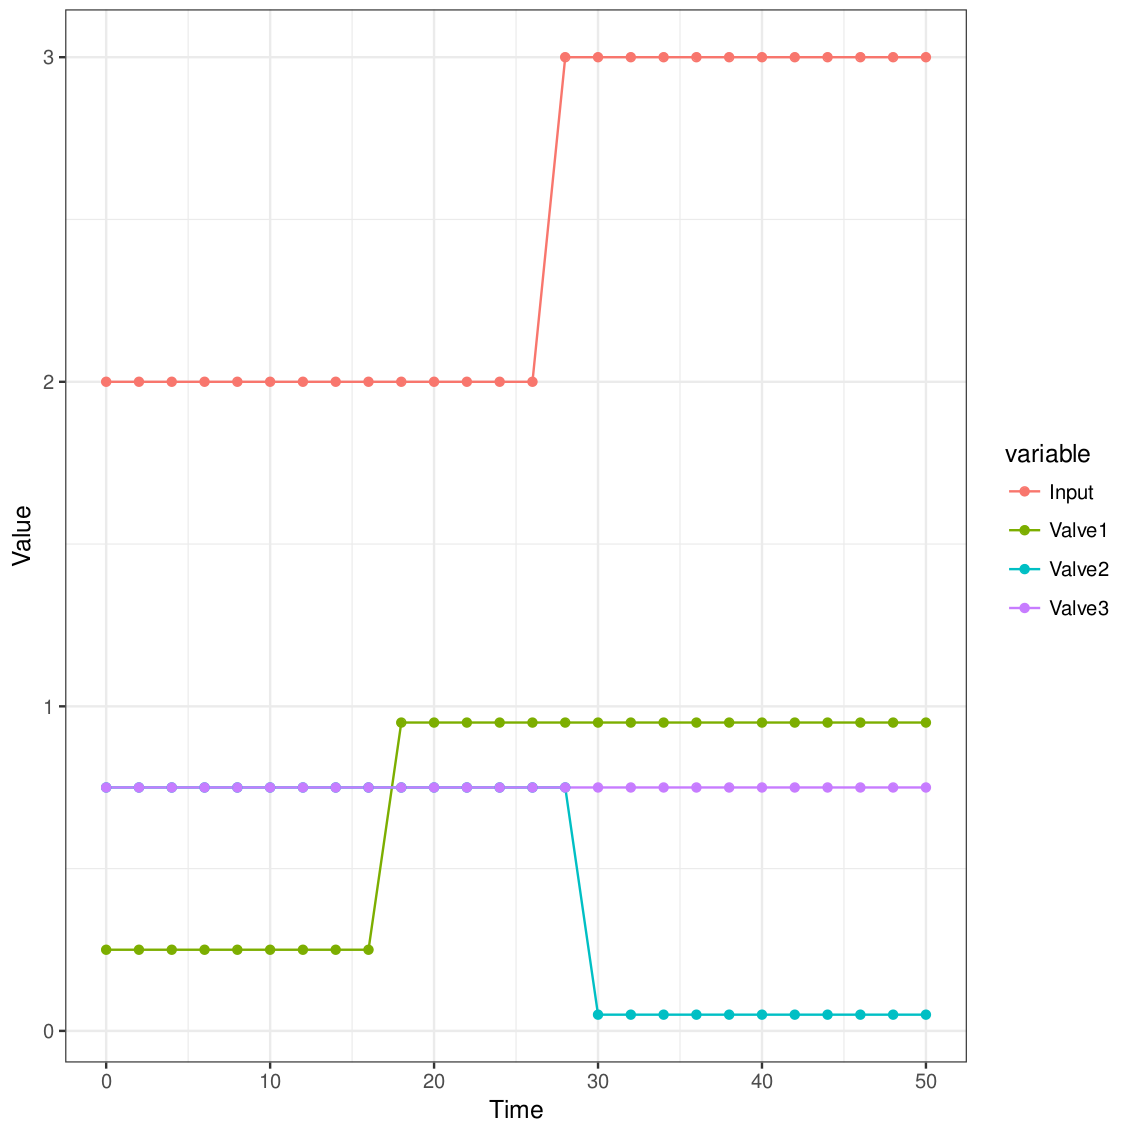
\includegraphics[width=0.5\textwidth]{issues_comb_input.png} &
			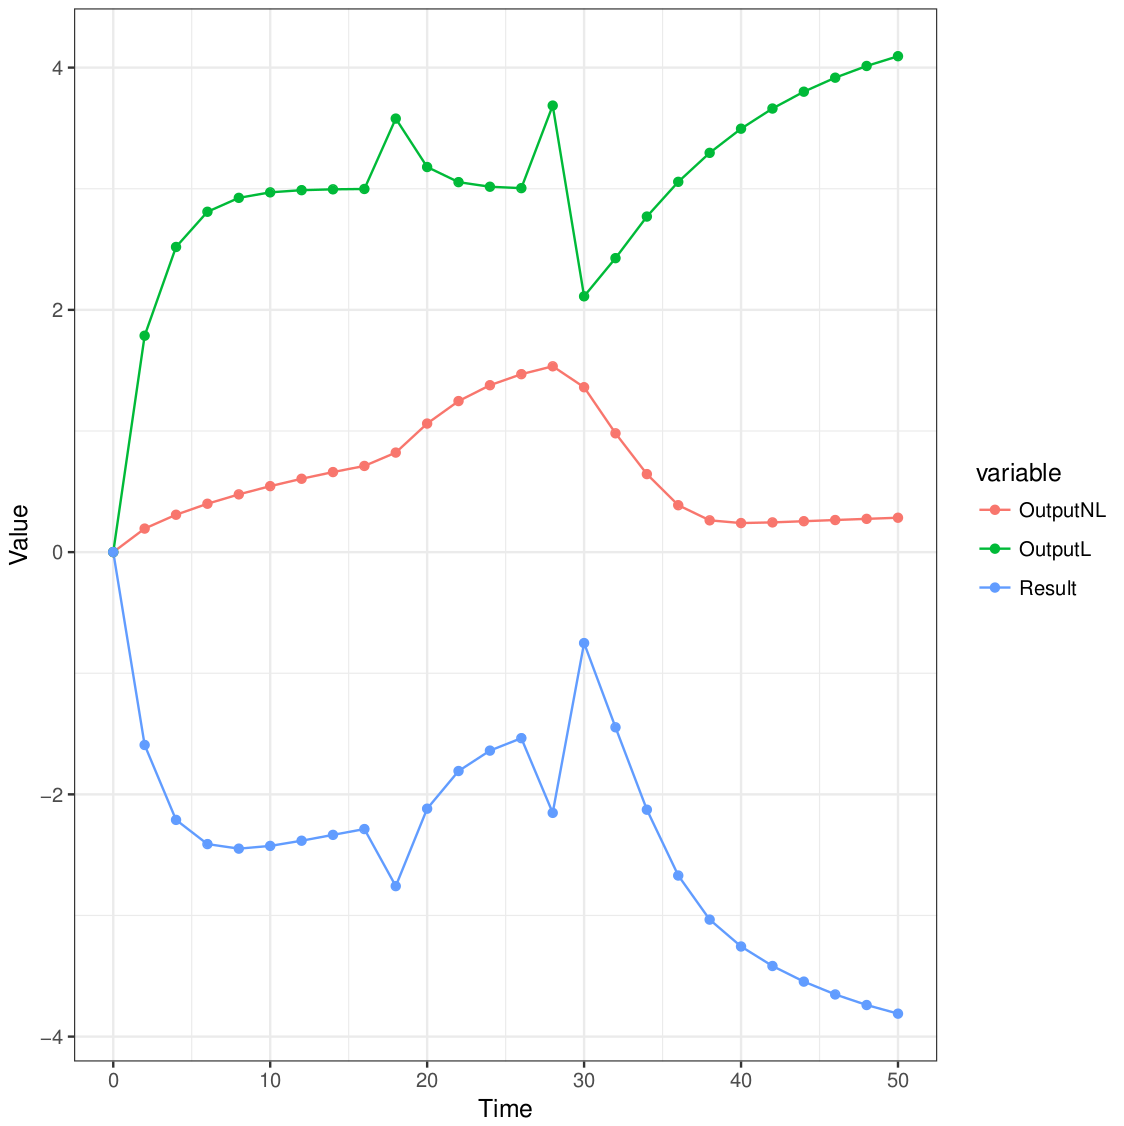
\includegraphics[width=0.5\textwidth]{issues_comb_output.png} \\
		\end{tabular}
	\end{table}
\end{frame}

\begin{frame}{Best corrective function}
	\begin{itemize}[<+->]
		\item[] Can we find the best corrective function for our linear model?
		\itemizespace%

		\item[] We are looking for a corrective function that could work in
		anytime for anything
		\itemizespace%
	\end{itemize}
\end{frame}

\begin{frame}{``Best'' for..}
	Combine different corrective function and find the optimal between them
	\begin{table}
		\begin{tabular}{ cc }
			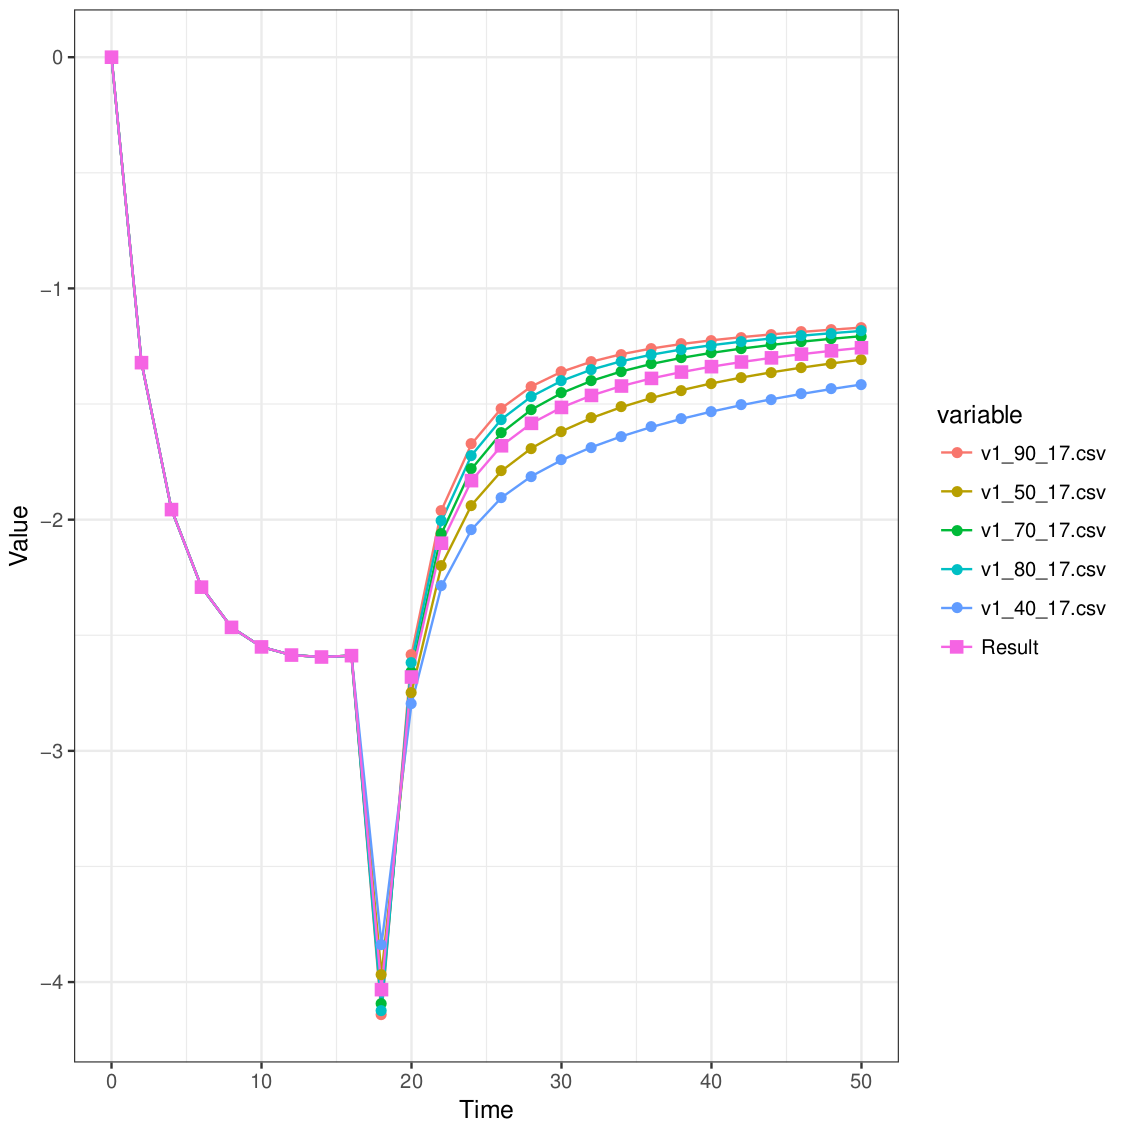
\includegraphics[width=0.5\textwidth]{multi_issues_v1_correction.png} &
			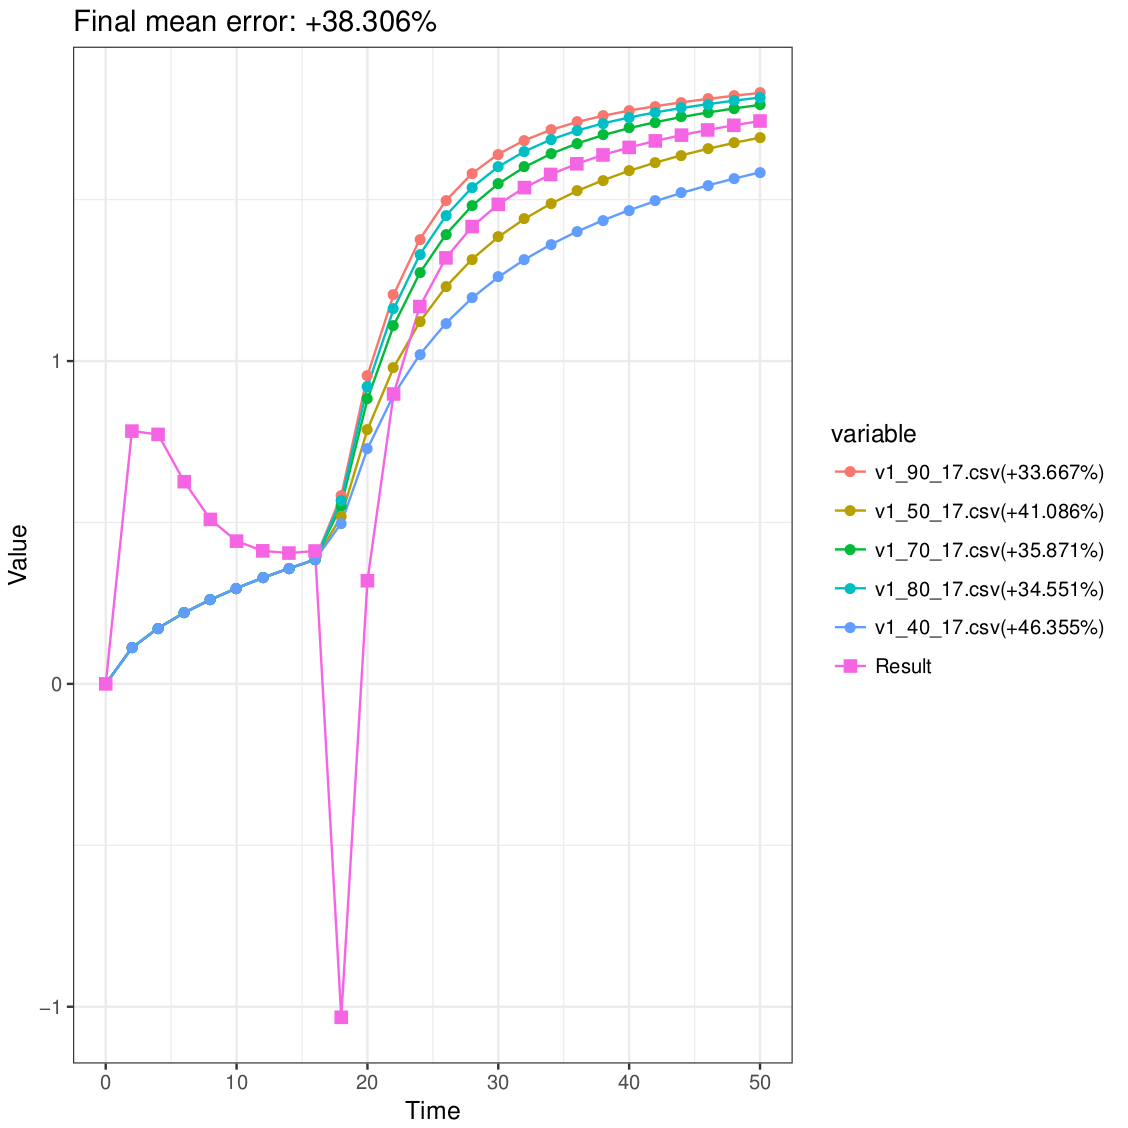
\includegraphics[width=0.5\textwidth]{multi_issues_v1_result.png} \\
		\end{tabular}
	\end{table}
\end{frame}

\begin{frame}{``Best'' for..}
	\begin{table}
		\begin{tabular}{ cc }
			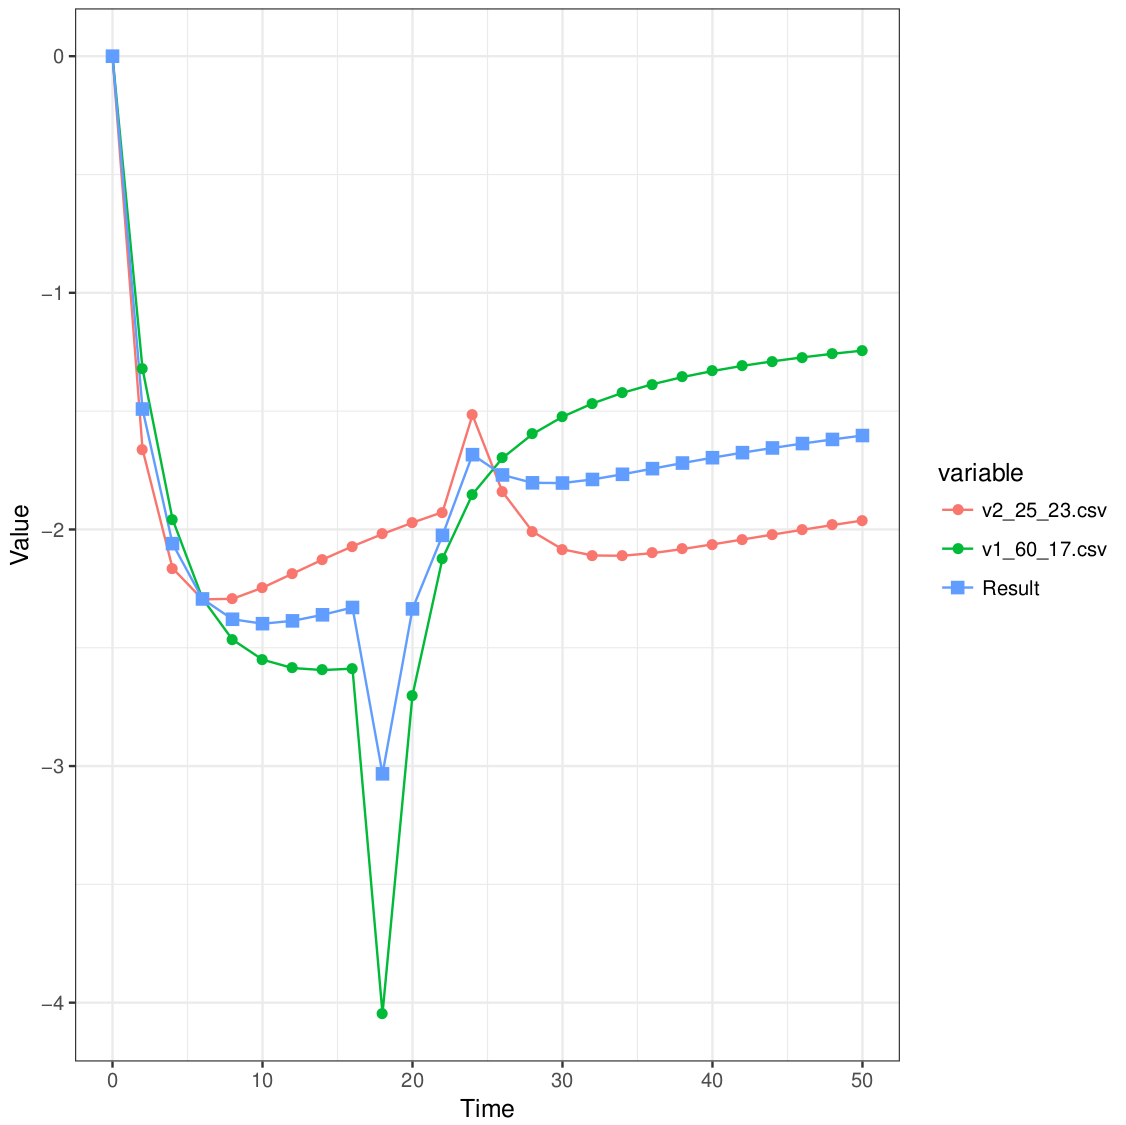
\includegraphics[width=0.5\textwidth]{multi_2_correction.png} &
			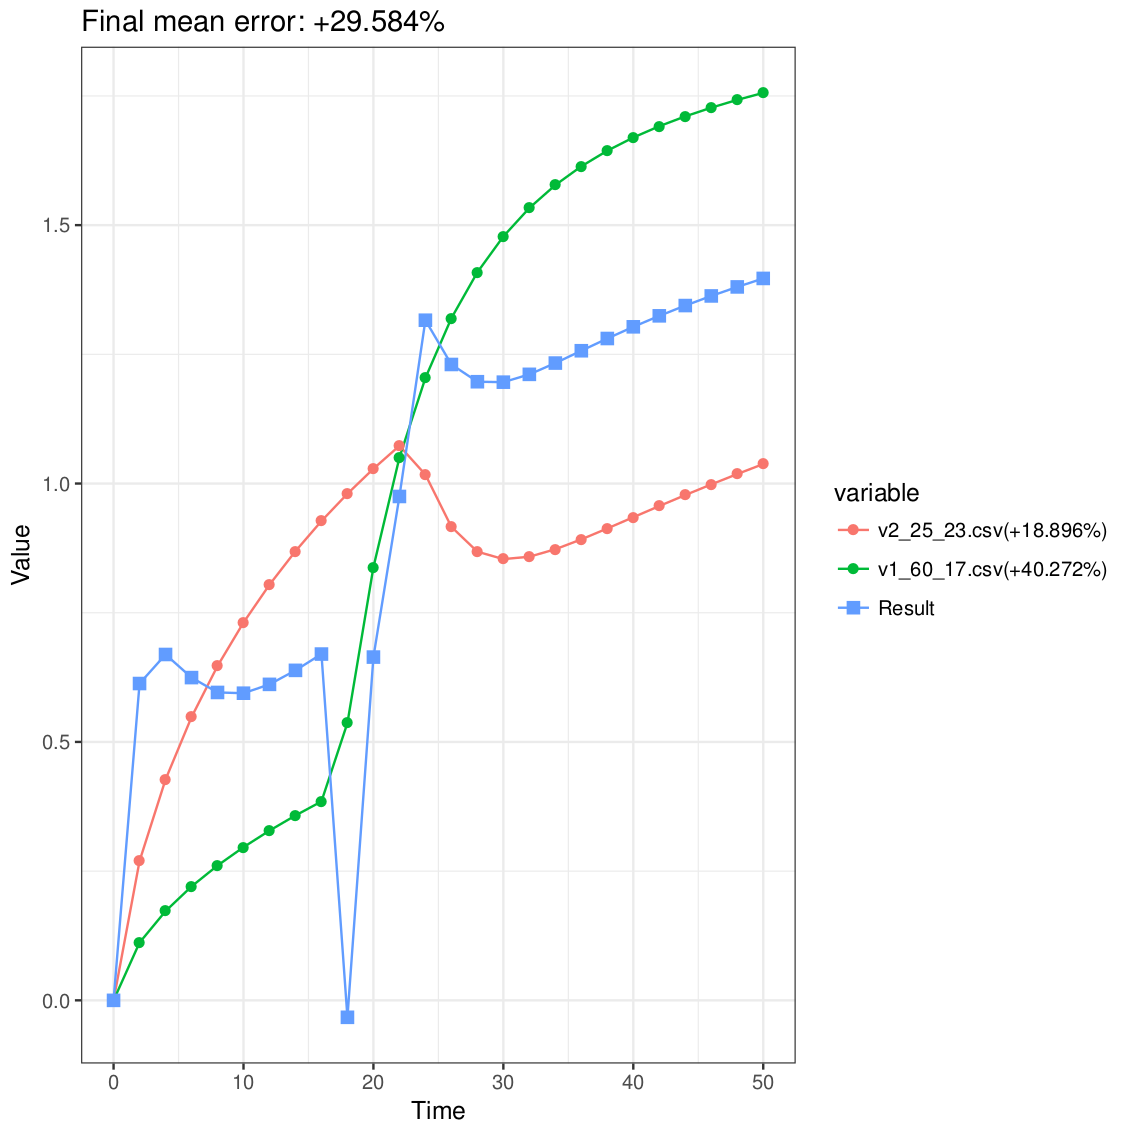
\includegraphics[width=0.5\textwidth]{multi_2_result.png} \\
		\end{tabular}
	\end{table}
\end{frame}

\begin{frame}{``Best'' for..}
	\begin{table}
		\begin{tabular}{ cc }
			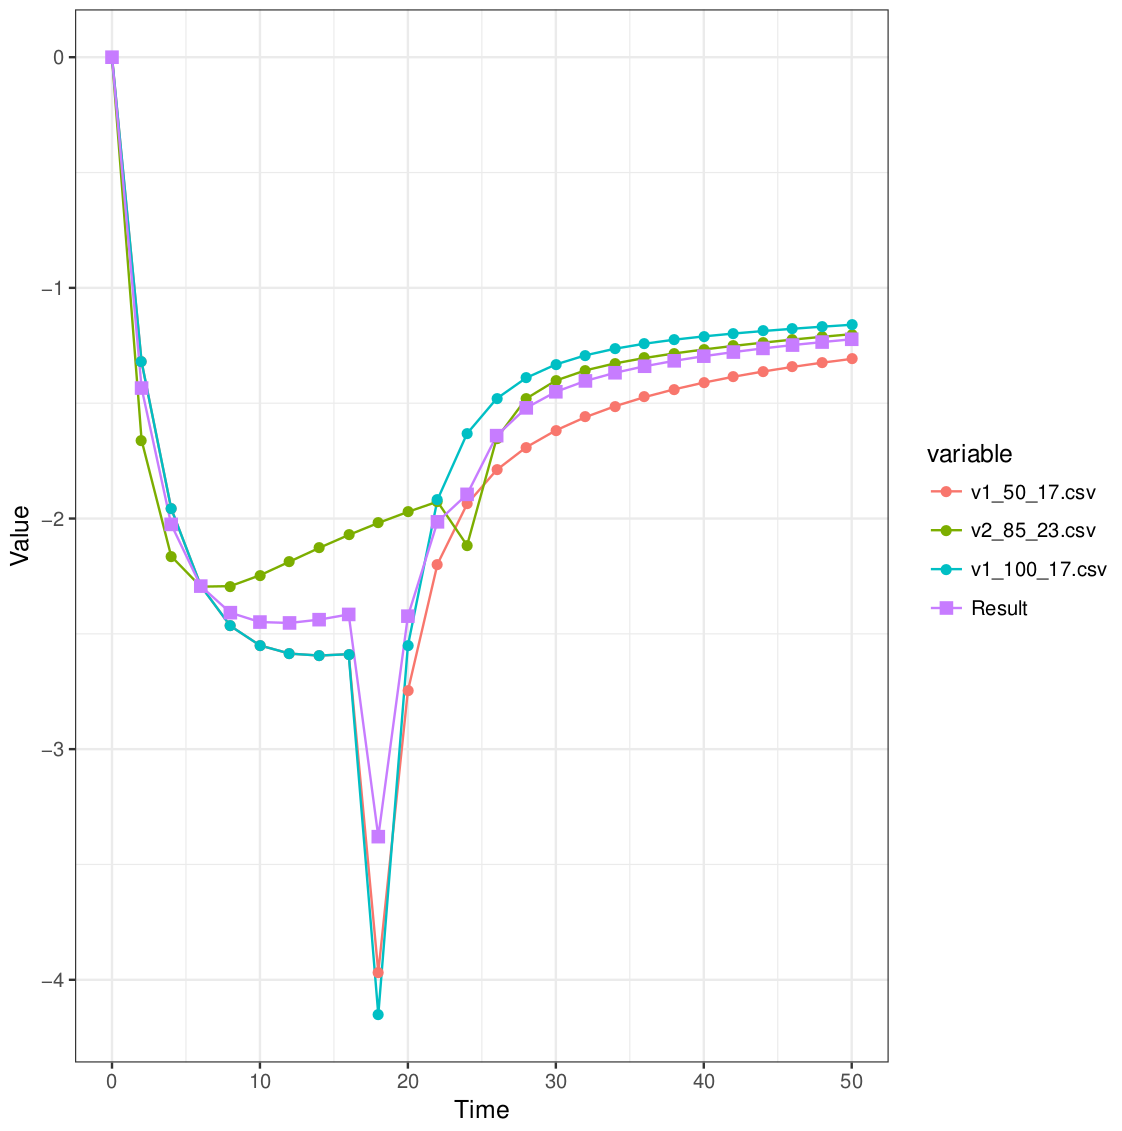
\includegraphics[width=0.5\textwidth]{multi_3_correction.png} &
			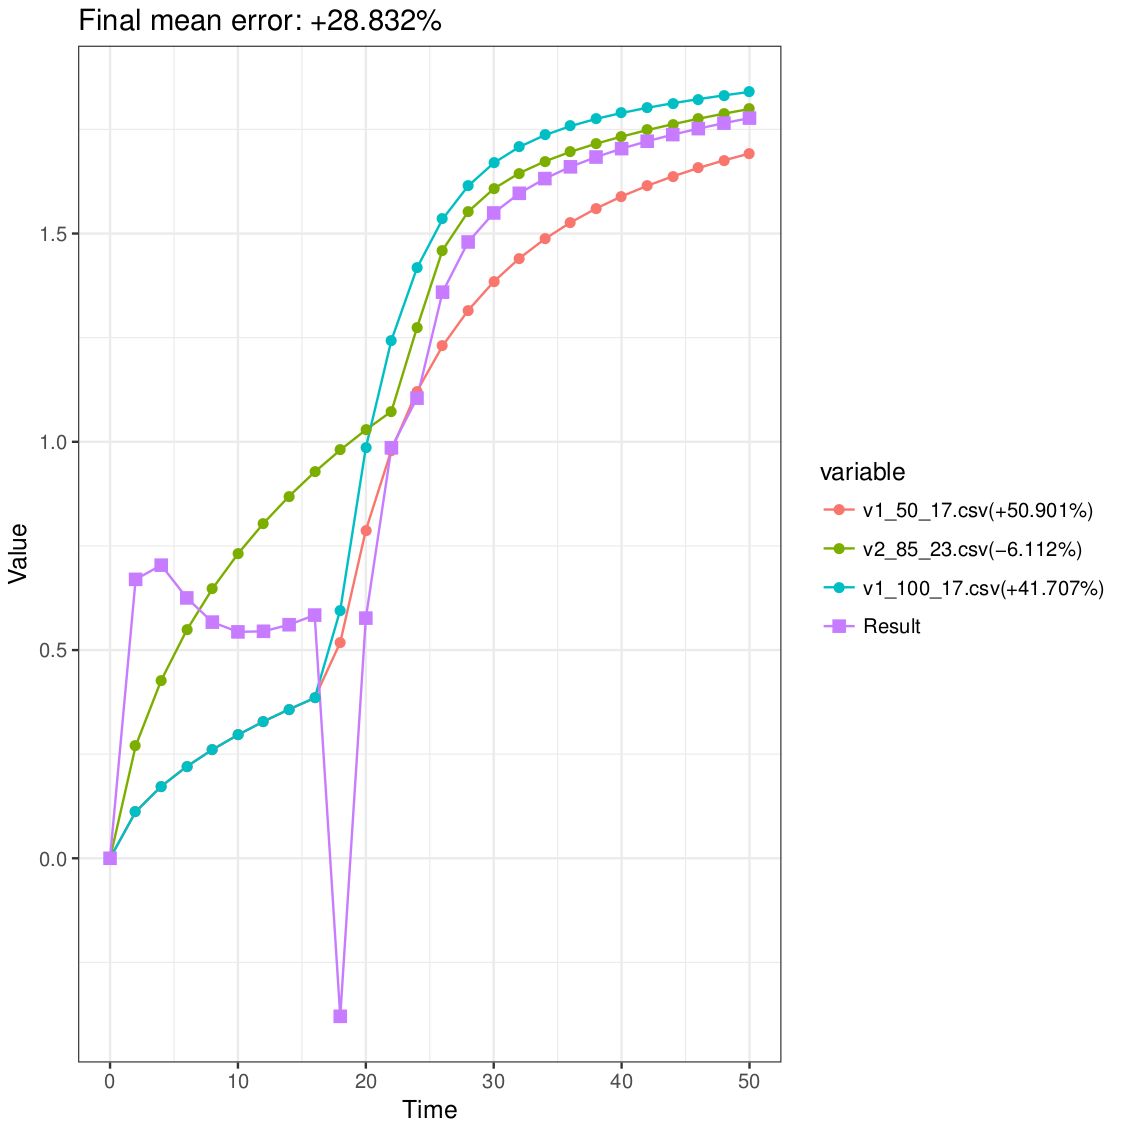
\includegraphics[width=0.5\textwidth]{multi_3_result.png} \\
		\end{tabular}
	\end{table}
\end{frame}

\begin{frame}{``Best'' for..}
	\begin{table}
		\begin{tabular}{ cc }
			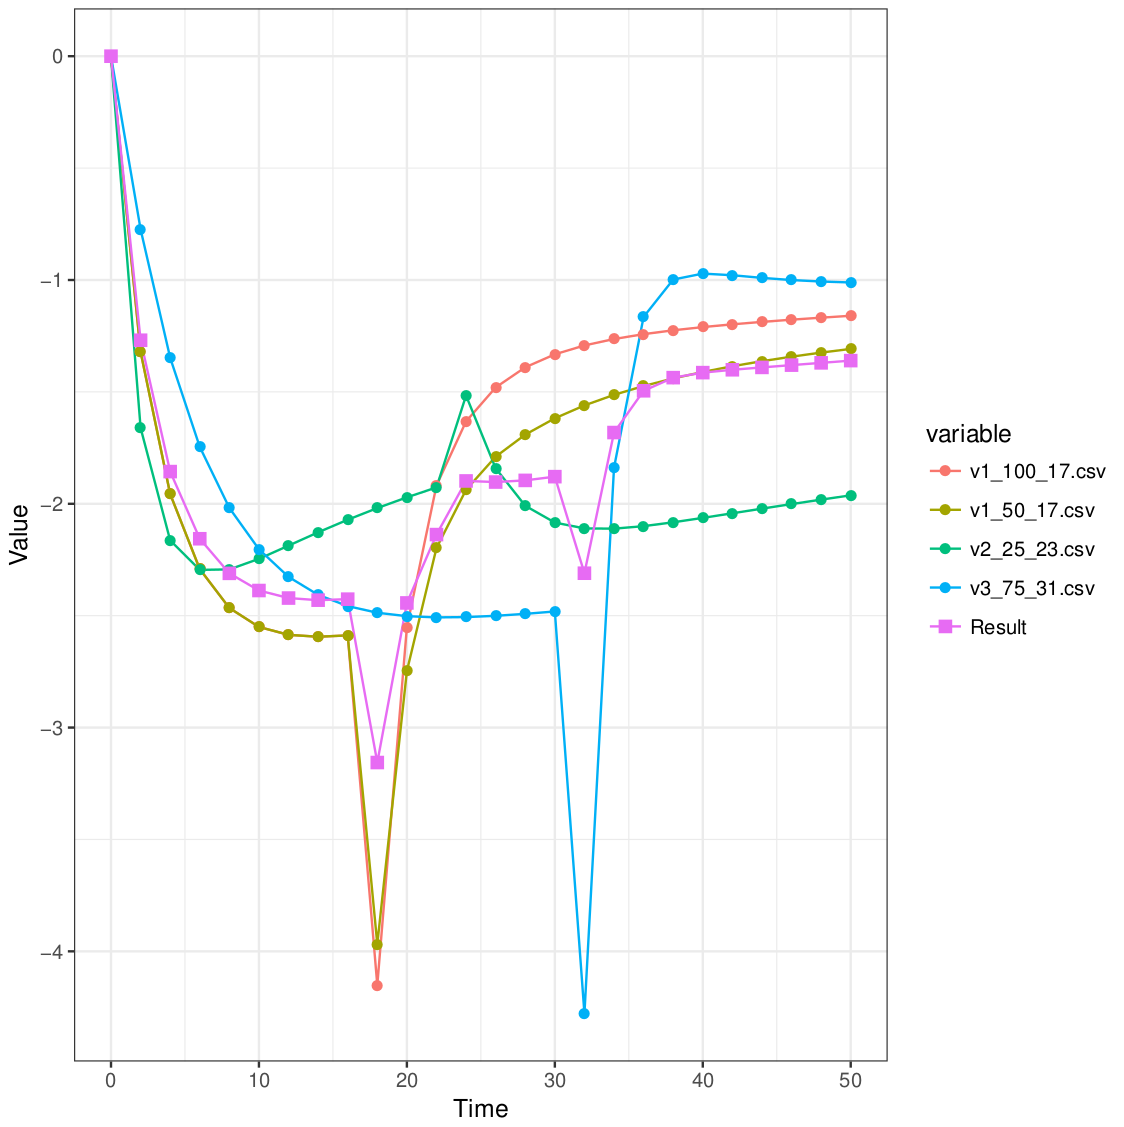
\includegraphics[width=0.5\textwidth]{multi_4_correction.png} &
			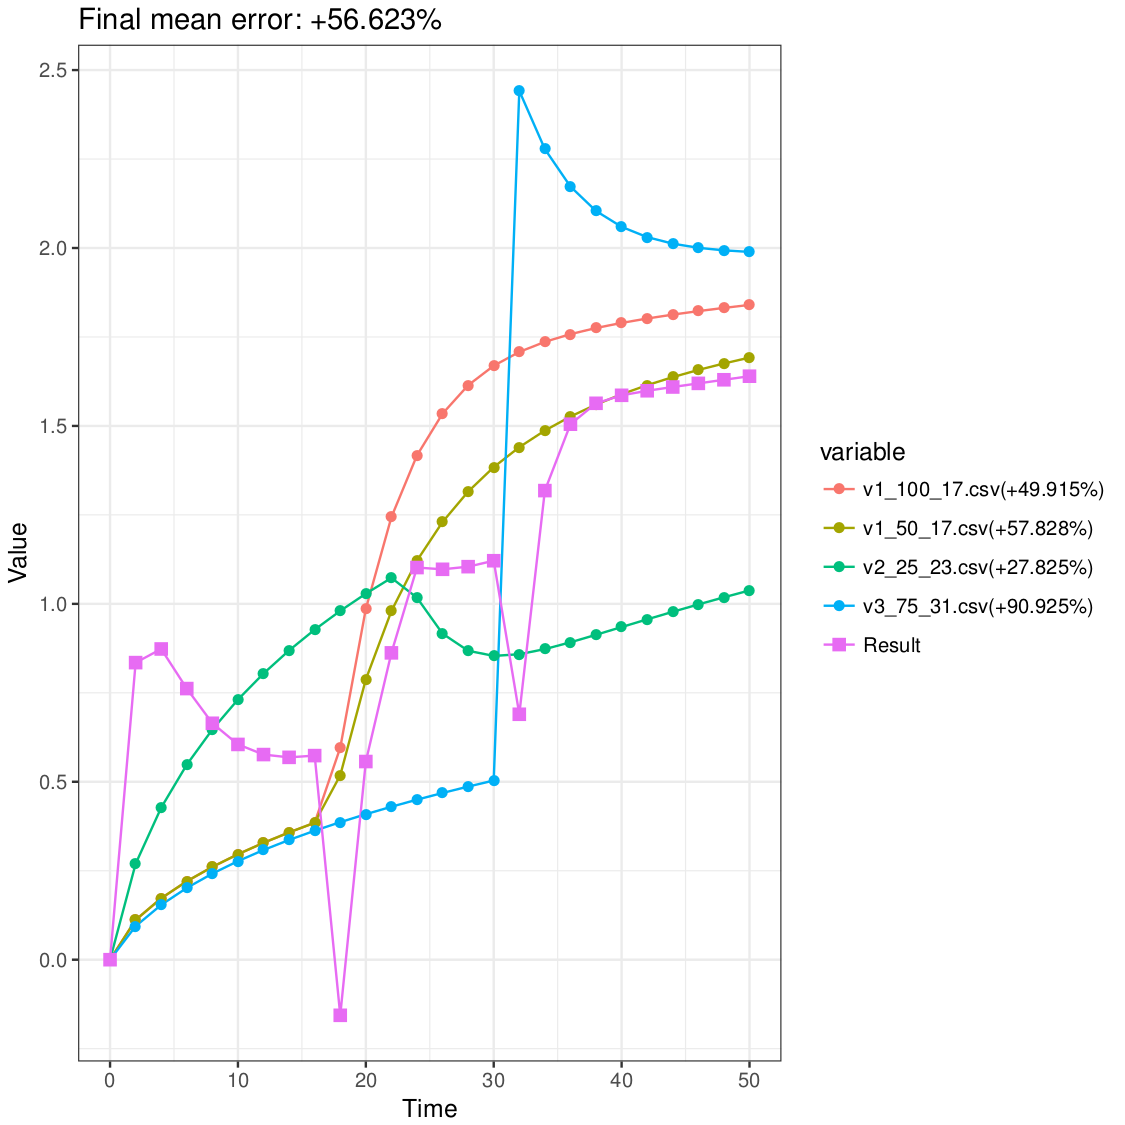
\includegraphics[width=0.5\textwidth]{multi_4_result.png} \\
		\end{tabular}
	\end{table}
\end{frame}

\subsection{Observations}
\begin{frame}{Observations}
	\begin{itemize}[<+->]
		\item[-] Multi issues independent
		\itemizespace%

		\item[-] Initial adapting time
		\itemizespace%

		\item[-] Require smoothing on spikes

	\end{itemize}
\end{frame}

\section{Diagnosis}
\subsection{Idea}
\begin{frame}{Diagnosis}
	Reversing the process and try to understand which issue has arisen knowing
	how the surrogate model behaved in that scenario
	
	\itemizespace%

	\begin{description}[<2->]
		\item[Series of SVM:]train an SVM for each known problem and use it
			to identify it when it occurs
		\itemizespace%

		\item[Neural Network]
	\end{description}
\end{frame}

\section{}
\begin{frame}
	\begin{figure}
		\centering
		
\includegraphics[height=0.4\textheight]{thank-you.jpg}
	\end{figure}
\end{frame}

\end{document}

